\section{Editar Datos Personales}

Los datos al pasar el tiempo son flexibles al cambio, esto quiere decir que un usuario que inicialmente sólo tenía un rol, ahora puede tener uno ó dos mas. De igual manera el peso, la altura, el correo electrónico e incluso la contraseña se pueden ver afectadas por el tiempo y es necesario actualizar estos datos.

\subsubsection{Procedimiento}
\begin{enumerate}
	
	\item Da clic en el icono \textbf{Editar Información} de la pantalla \textbf{Datos Principales}.

	\item Se mostrará la pantalla \textbf{Editar Información}.
	
	\begin{figure}[!htbp]
		\hypertarget{fig:editInfo}{\hspace{1pt}}
		\begin{center}
			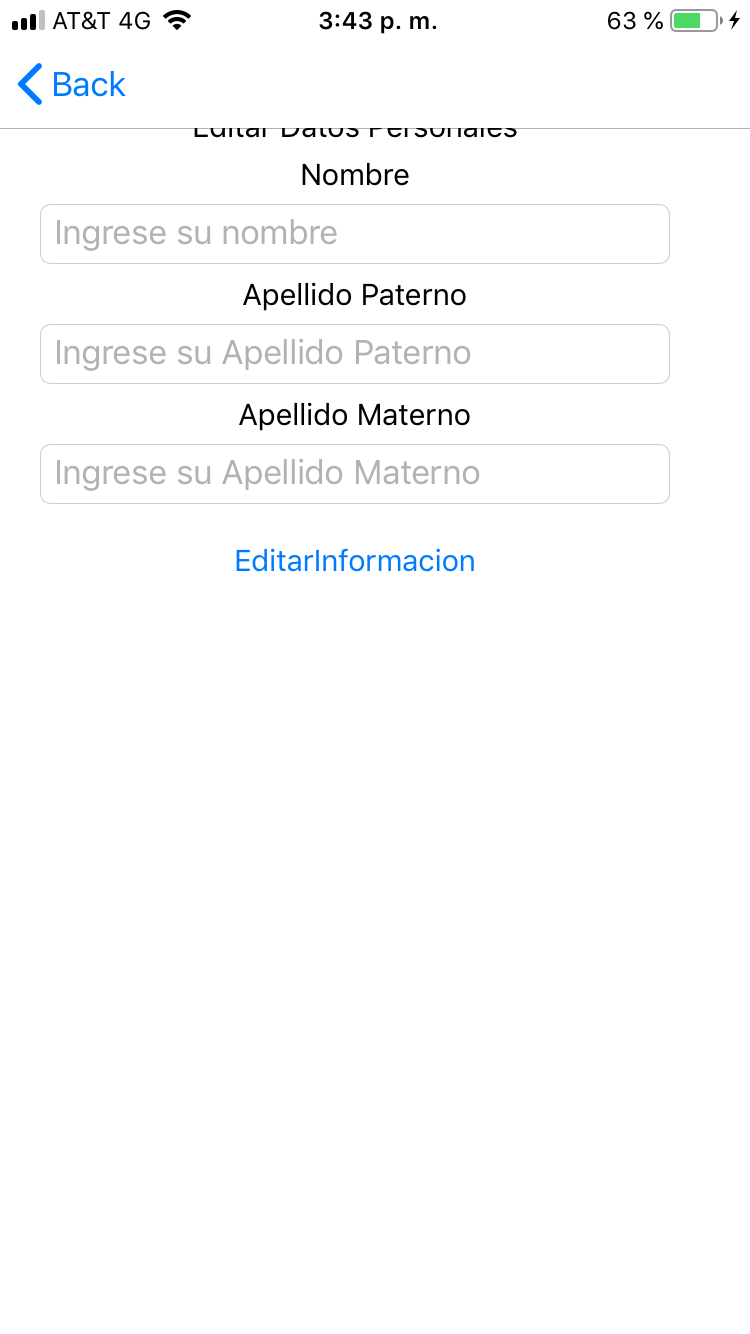
\includegraphics[height=0.4\textheight]{Doctor/EditarDP/images/editInfo}
			\caption{Editar Información}
			\label{fig:editInfo}
		\end{center}
	\end{figure}

	\item Edita la información que consideres necesaria.
	
	\item Presiona el botón \textbf{Editar Información} para guardar los cambios de tus datos personales.

\end{enumerate}

